\documentclass[12pt, letterpaper, preprint]{aastex}
%%% This file is generated by the Makefile.
\newcommand{\giturl}{\url{https://github.com/changhoonhahn/feasiBGS}}
\newcommand{\githash}{e930d31}\newcommand{\gitdate}{2018-04-13}\newcommand{\gitauthor}{ChangHoon Hahn}

\usepackage[breaklinks,colorlinks, urlcolor=blue,citecolor=blue,linkcolor=blue]{hyperref}
\usepackage{color}
\usepackage{amsmath}
\usepackage{natbib}
\usepackage{ctable}
\usepackage{bm}
\usepackage[normalem]{ulem} % Added by MS for \sout -> not required for final version
\usepackage{xspace}

% typesetting shih
\linespread{1.08} % close to 10/13 spacing
\setlength{\parindent}{1.08\baselineskip} % Bringhurst
\setlength{\parskip}{0ex}
\let\oldbibliography\thebibliography % killin' me.
\renewcommand{\thebibliography}[1]{%
  \oldbibliography{#1}%
  \setlength{\itemsep}{0pt}%
  \setlength{\parsep}{0pt}%
  \setlength{\parskip}{0pt}%
  \setlength{\bibsep}{0ex}
  \raggedright
}
\setlength{\footnotesep}{0ex} % seriously?

% citation alias

% math shih
\newcommand{\setof}[1]{\left\{{#1}\right\}}
\newcommand{\given}{\,|\,}
\newcommand{\pseudo}{{\mathrm{pseudo}}}
\newcommand{\Var}{\mathrm{Var}}
\newcommand{\Nd}{{100}\xspace}

\newcommand{\specialcell}[2][c]{%
  \begin{tabular}[#1]{@{}c@{}}#2\end{tabular}}
% text shih
\newcommand{\foreign}[1]{\textsl{#1}}
\newcommand{\etal}{\foreign{et~al.}}
\newcommand{\opcit}{\foreign{Op.~cit.}}
\newcommand{\documentname}{\textsl{Article}}
\newcommand{\equationname}{equation}
\newcommand{\bitem}{\begin{itemize}}
\newcommand{\eitem}{\end{itemize}}
\newcommand{\beq}{\begin{equation}}
\newcommand{\eeq}{\end{equation}}

%% MS: To make collaborating easier
\definecolor{orange}{rgb}{1,0.5,0}
\setlength{\marginparwidth}{1.2in}
\let\oldmarginpar\marginpar
\renewcommand\marginpar[1]{\-\oldmarginpar[\raggedleft\footnotesize #1]%
  {\raggedright\footnotesize #1}}

%%% Here are the things that make collaborative effort easier
\newcommand{\todo}[1]{\marginpar{\color{red}TODO}{\color{red}#1}}
\newcommand{\ab}[1]{{\color{blue}{\bf AB:} #1}}
\newcommand{\ms}[1]{{\color{orange}{\bf MS:}} {[\em #1}]}

%% MS: Latex shortcuts
\newcommand{\lss}{{\small{LSS}}\xspace}
\newcommand{\gmm}{{\small{GMM}}\xspace}
\newcommand{\gmms}{{\small{GMM}s}\xspace}
\newcommand{\EM}{{\small{EM}}\xspace}
\newcommand{\bic}{{\small{BIC}}\xspace}
\newcommand{\pca}{{\small{PCA}}\xspace}
\newcommand{\ica}{{\small{ICA}}\xspace}

\newcommand{\patchy}{{\fontshape\scdefault\selectfont patchy}}

\begin{document}\sloppy\sloppypar\frenchspacing 

\title{Feasibility of DESI: Bright Galaxy Survey}
\date{\texttt{DRAFT~---~\githash~---~\gitdate~---~NOT READY FOR DISTRIBUTION}}


\newcounter{affilcounter}
% \altaffiltext{1}{}

\setcounter{affilcounter}{1}

\edef \lbl {\arabic{affilcounter}}\stepcounter{affilcounter}
\altaffiltext{\lbl}{Lawrence Berkeley National Laboratory, 1 Cyclotron Rd, Berkeley CA 94720, USA}

\edef \bccp {\arabic{affilcounter}}\stepcounter{affilcounter}
\altaffiltext{\bccp}{Berkeley Center for Cosmological Physics, University of California, Berkeley, CA 94720, USA}

\author{
    ChangHoon~Hahn\altaffilmark{\lbl, \bccp}, 
    David~Schlegel\altaffilmark{\lbl}
}
\email{changhoon.hahn@lbl.gov}

\begin{abstract}
testing 
\end{abstract}

\keywords{
cosmology: observations
---
}

\section{Introduction}

%%%%%%%%%%%%%%%%%%%%%%%%%%%%%%%%%%%%%
% Figure  
%%%%%%%%%%%%%%%%%%%%%%%%%%%%%%%%%%%%%
\begin{figure}
\begin{center}
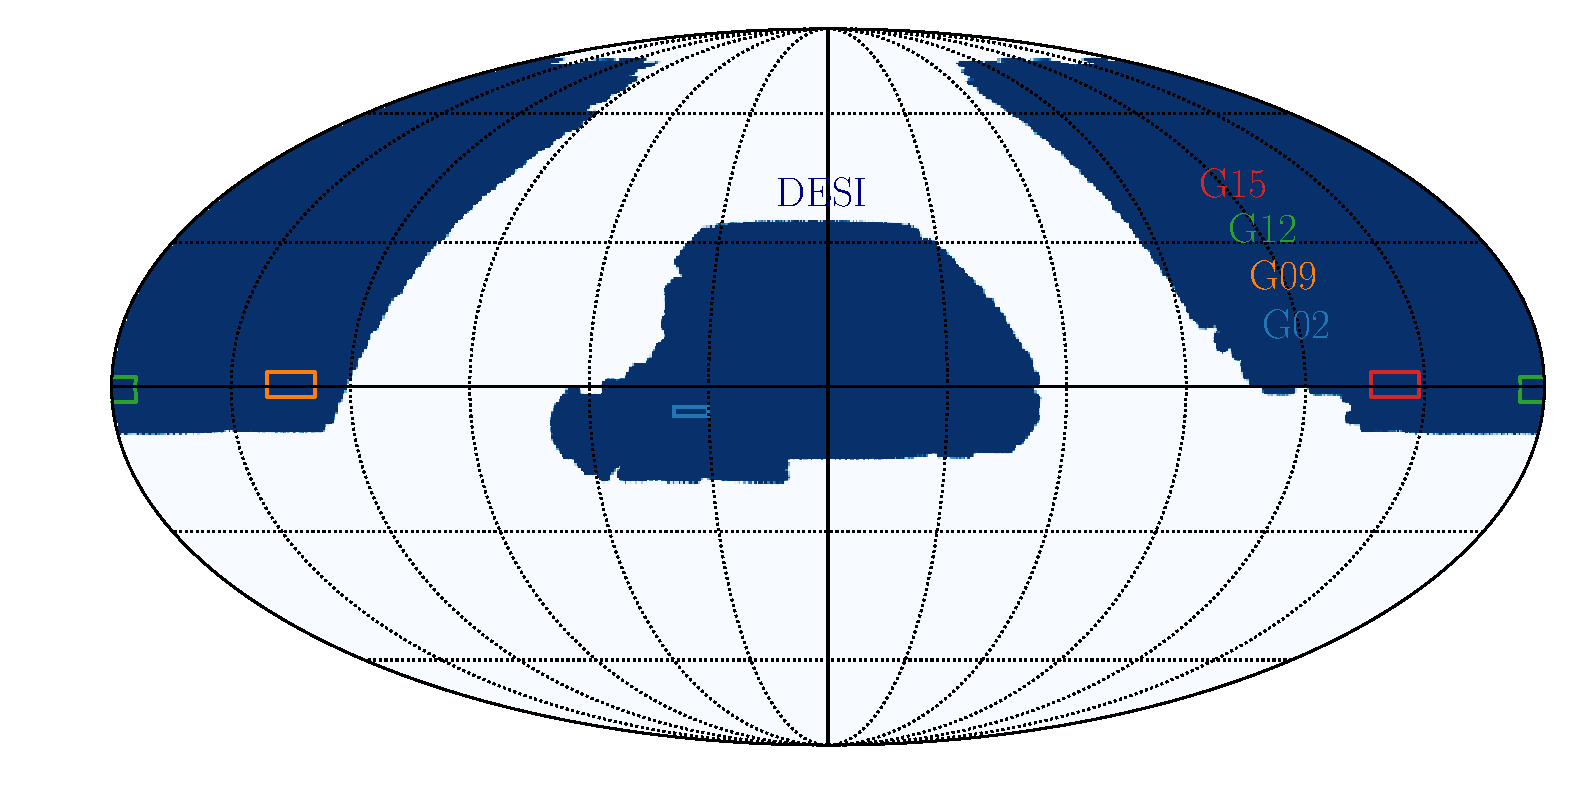
\includegraphics[width=0.7\textwidth]{figs/DESI_GAMA.pdf}
    \caption{Footprint of GAMA DR2 (orange) overplotted on 
    the DESI footprint (blue). This highlight that the GAMA 
    galaxies are within the DESI footprint. This makes them
    an excellent sample to assess the feasibility of BGS.}
\label{fig:desigama_footprint}
\end{center}
\end{figure}
%%%%%%%%%%%%%%%%%%%%%%%%%%%%%%%%%%%%%

%%%%%%%%%%%%%%%%%%%%%%%%%%%%%%%%%%%%%
% Figure  
%%%%%%%%%%%%%%%%%%%%%%%%%%%%%%%%%%%%%
\begin{figure}
\begin{center}
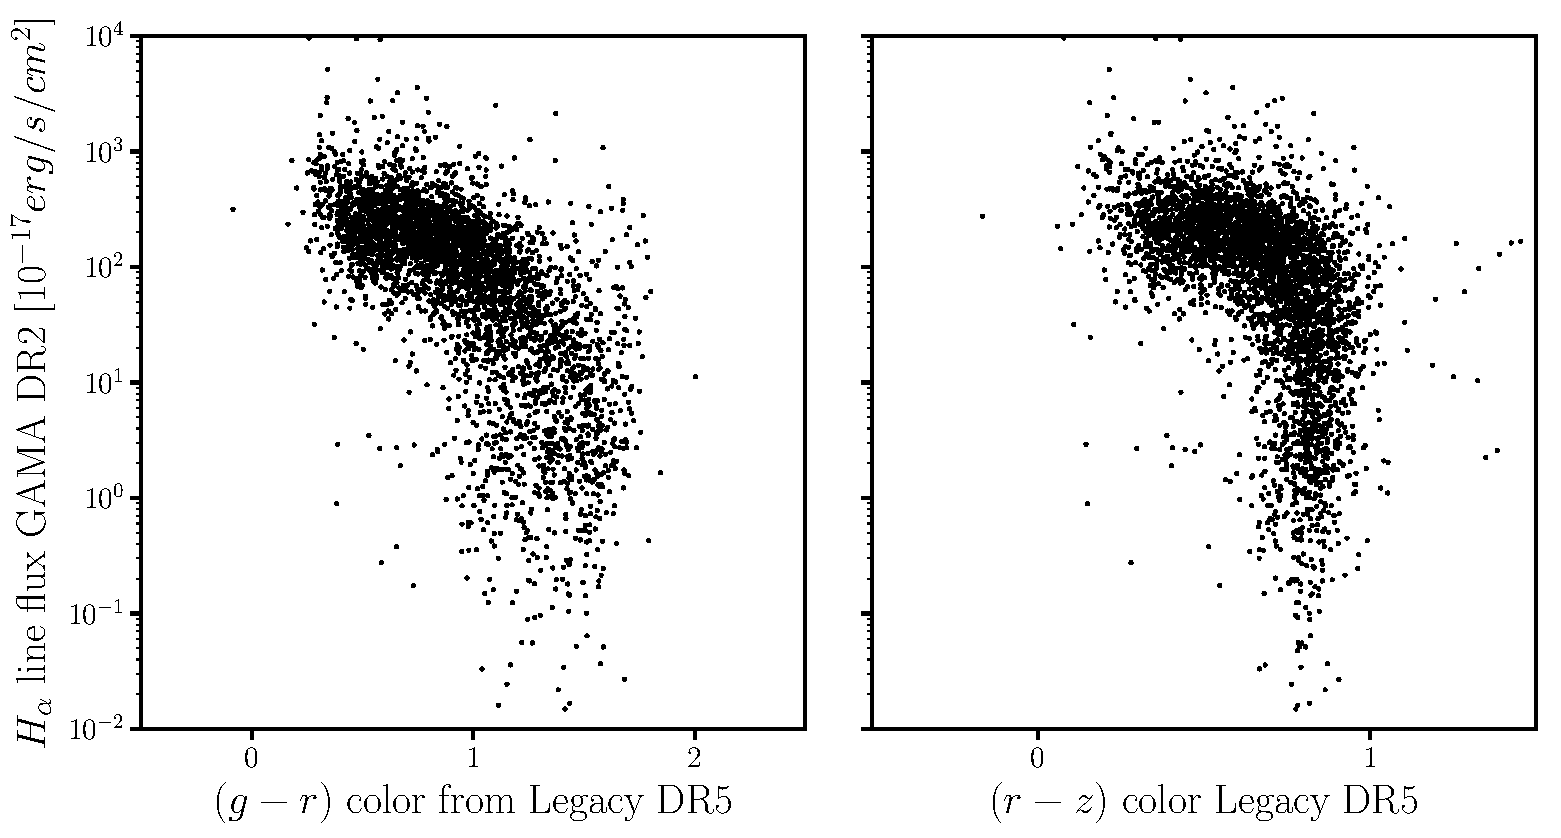
\includegraphics[width=0.7\textwidth]{figs/GAMALegacy_Halpha_color.pdf}
    \caption{$(g - r)$ and $(r - z)$ colors to $H_\alpha$ line flux 
    relations for galaxies that are in both the GAMA DR 2 and the 
    Legacy survey DR 5. The $(g - r)$ and $(r - z)$ colors are calculated
    from the Legacy survey DR 5 model flux. Meanwhile the $H_\alpha$ line 
    flux is from the GAMA DR 2, where they fit a Gaussian to the emission 
    line. For convenience, the galaxy sample is downsampled by a factor of 
    $10$.}
\label{fig:desigama_footprint}
\end{center}
\end{figure}
%%%%%%%%%%%%%%%%%%%%%%%%%%%%%%%%%%%%%

%%%%%%%%%%%%%%%%%%%%%%%%%%%%%%%%%%%%%
% Figure  
%%%%%%%%%%%%%%%%%%%%%%%%%%%%%%%%%%%%%
\begin{figure}
\begin{center}
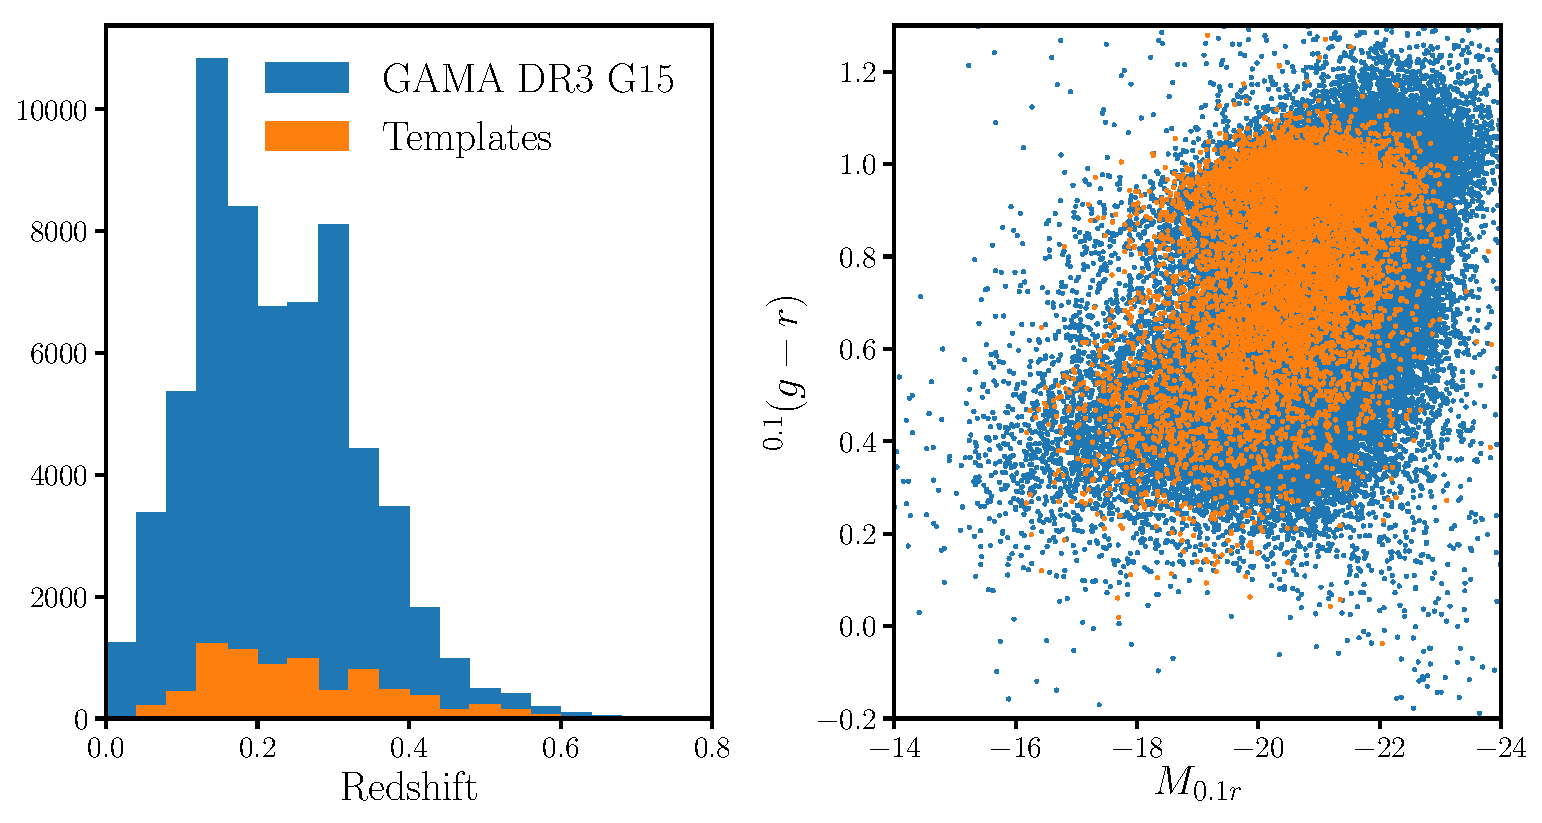
\includegraphics[width=0.7\textwidth]{figs/BGStemplates.pdf}
    \caption{Properties of the $7636$ BGS templates. The left 
    is the redshift distribution of the templates while the right
    plots the $M_r$ versus $(g - r)$ color magnitude relation of 
    the templates. Both $M_r$ and $(g-r)$ values are $k$-corrected 
    to $z = 0.1$.}
\label{fig:bgstemp_meta}
\end{center}
\end{figure}
%%%%%%%%%%%%%%%%%%%%%%%%%%%%%%%%%%%%%

%%%%%%%%%%%%%%%%%%%%%%%%%%%%%%%%%%%%%
% Figure  
%%%%%%%%%%%%%%%%%%%%%%%%%%%%%%%%%%%%%
\begin{figure}
\begin{center}
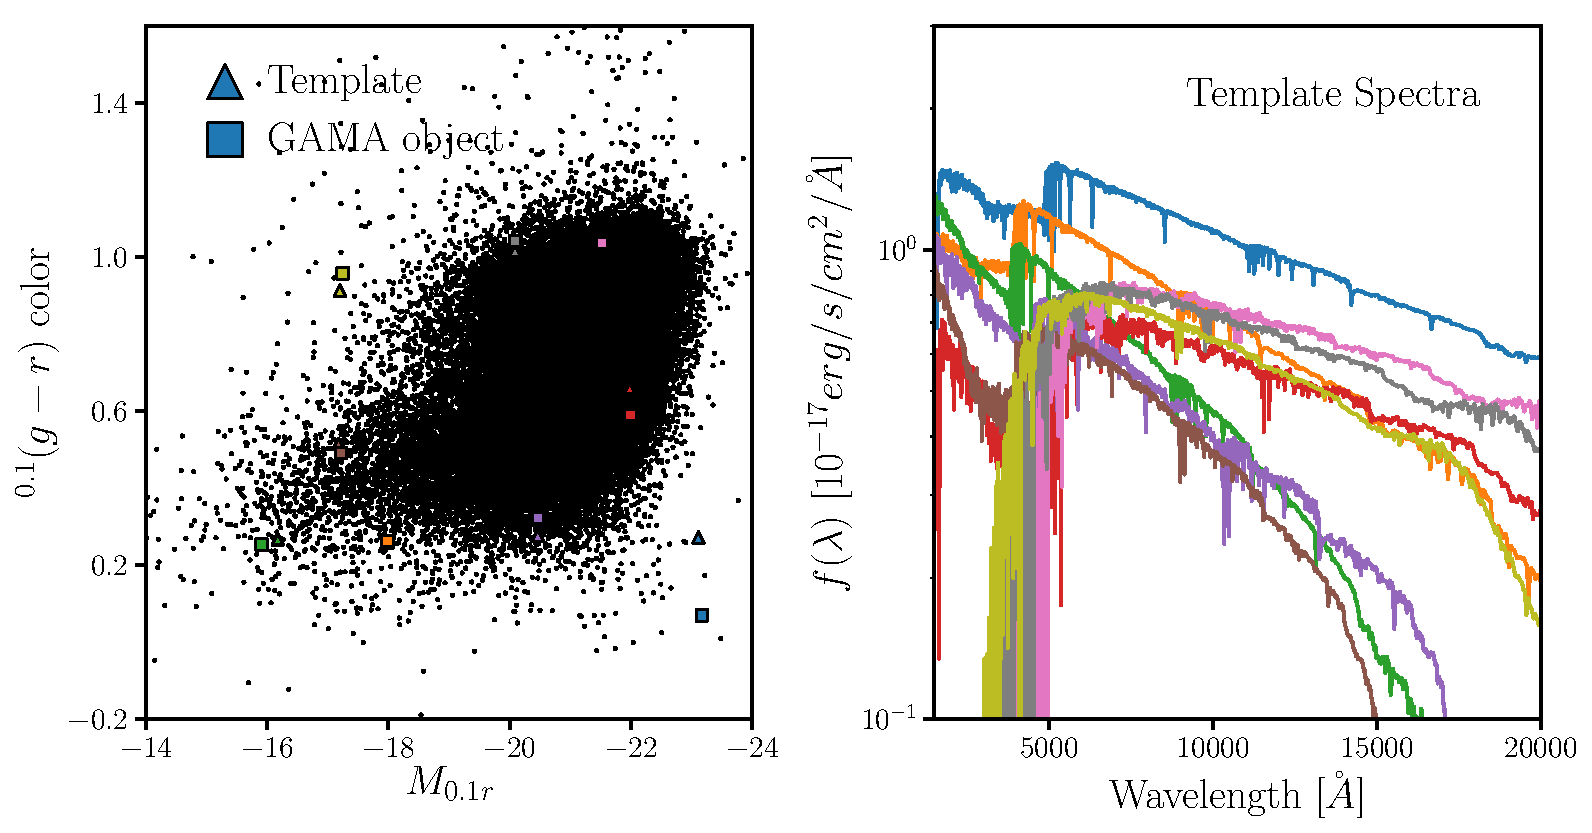
\includegraphics[width=0.7\textwidth]{figs/GamaLegacy_matchedtempSpectra.pdf}
    \caption{A handful of GAMA DR2 galaxies are randomly selected then 
    matched to templates with the closest redshift, $r$ band absolute 
    magnitude ($M_{0.1,r}$), and $^{0.1}(g - r)$ color. The left panel
    plots the $M_{0.1,r}$) to $^{0.1}(g - r)$ color relation of the GAMA
    DR2 galaxies with the randomly selected galaxies highlighted (square). 
    The matched templates are marked with same color (triangle). In the 
    right panel, spectra for the match templates are plotted in the same 
    color.}
\label{fig:temp_spectra}
\end{center}
\end{figure}
%%%%%%%%%%%%%%%%%%%%%%%%%%%%%%%%%%%%%
%\bibliographystyle{yahapj}
\end{document}
